\documentclass{article}
\usepackage{iclr2027_conference,times}

\usepackage{amsmath,amssymb,amsthm}
\usepackage{booktabs}
\usepackage{multirow}
\usepackage{graphicx}
\usepackage{microtype}
\usepackage[most]{tcolorbox}
\usepackage{xcolor}
\usepackage[colorlinks=true,linkcolor=blue,citecolor=blue]{hyperref}
\usepackage{url}

% ---------------------------------------------------------------- macros ----
\newcommand{\E}{\mathbb{E}}
\newcommand{\ind}[1]{\mathbf{1}\!\left[#1\right]}
\newcommand{\sg}{\mathrm{sg}}
\newcommand{\cube}{c}
\newcommand{\BRR}{\textsc{BRR}}
\newcommand{\Reach}{\mathrm{reach}}
\newcommand{\Visit}{\mathrm{visit}}

\newtheorem{proposition}{Proposition}

\definecolor{findingframe}{HTML}{2F4858}
\definecolor{findingback}{HTML}{F2F6F8}
\newtcolorbox{finding}[1][]{
  enhanced, breakable,
  colback=findingback, colframe=findingframe,
  boxrule=0.4pt, left=6pt, right=6pt, top=5pt, bottom=5pt,
  fonttitle=\bfseries\footnotesize,
  coltitle=white,
  attach boxed title to top left={yshift=-2mm, xshift=4mm},
  boxed title style={colback=findingframe, boxrule=0pt, sharp corners},
  title={Finding}, #1
}

\title{Making Successor Measures Work for Robot Manipulation}
\author{Anonymous}

% Uncomment for the camera-ready version.
% \iclrfinalcopy

\begin{document}
\maketitle

\begin{abstract}
Successor measures promise a single dynamics-dependent representation that can be
reused for any reward. Yet standard forward--backward representations perform
poorly on offline robot manipulation, even when a goal-conditioned method with the
same data, actor class, and bilinear critic succeeds. We trace this gap to the
estimator rather than to the representation. The pointwise successor-density
Bellman equation contains a singular immediate term. Standard FB replaces it with
an unmatched linear term whose scale is controlled by an orthonormality penalty.
On a frozen embedding that already supports $0.97$ task success, removing that
penalty sends the critic scale from $154$ to $5.4\times 10^4$ and degrades control
to $0.42$. Retaining the penalty stabilizes scale but suppresses control. We
replace point queries with bounded, task-aligned regions, turning the singular
term into a binary event and the full objective into ordinary Bellman regression.
The resulting reaching value obtains $0.967$, $0.549$, and $0.484$ success on
OGBench \texttt{cube-single}, \texttt{cube-double}, and \texttt{scene}, compared
with $0.928$, $0.265$, and $0.281$ for a matched goal-conditioned IQL anchor. A
visitation extension predicts coarse discounted set mass and earns $1.33\times$
the return of the reaching object on unseen rewards, but remains negative on
$45\%$ of state--goal pairs and loses control performance on harder environments.
The results separate three problems that are often conflated: learning
reachability, learning a valid measure, and training a policy that can act on
reward-derived task vectors.
\end{abstract}

% ============================================================================
\section{Introduction}
\label{sec:introduction}

A successor measure describes where a policy will go. Once this object is known,
a new reward can be evaluated by integration rather than by retraining a value
function. This is the main appeal of successor representations and
forward--backward (FB) methods: dynamics are learned once, while rewards can be
specified later \citep{dayan1993improving,touati2021learning,touati2023does}.
Robot play data appears to be a natural setting for this idea. A large offline
dataset may contain many ways of moving objects, and the reward of interest may
only be known after data collection.

In practice, the promise does not carry cleanly to manipulation. On OGBench
\texttt{cube-single-play-v0}, tuned FB variants plateau near $0.42$ overall
success, while goal-conditioned IQL reaches $0.93$ using the same data, actor
class, and bilinear critic architecture. The gap is not caused by online
exploration, because both methods learn from the same fixed dataset. It is also
not obviously caused by insufficient representational capacity, because the
successful goal-conditioned anchor uses the same low-rank form. This leaves a
more basic question:

\begin{quote}
\emph{What prevents a successor-measure objective from learning a useful object
when an almost identical goal-conditioned value function succeeds?}
\end{quote}

The key insight is that standard FB does not regress the successor-density
Bellman equation directly. The immediate term of that equation is a Dirac density
ratio. It has no finite scalar target at the observed successor. FB therefore uses
a density-matching surrogate in which random query states receive a squared
residual, while the matched successor receives a negative linear term. That
linear term rewards increasing the matched value without specifying where it
should stop. An orthonormality penalty on the backward representation becomes the
scale anchor. The estimator is then caught between two requirements: removing the
penalty allows scale to diverge, while retaining it imposes a geometry that can
harm control.

We test this diagnosis before proposing a new method. We freeze a backward map
from a checkpoint that already achieves $0.97$ success and train only the standard
density estimator. Its scale diverges and its control performance deteriorates.
Because the representation is fixed and already useful, this experiment localizes
the failure to the estimator. We then make one substitution: query a finite goal
region rather than a point. The singular immediate term becomes a binary hit
event. Every state--query pair, including the matched pair, now has an explicit
Bellman target. No separate linear term or orthonormality constraint is required.

This substitution produces two related objects. An absorbing backup learns the
discounted probability of first reaching a region. A nonabsorbing backup learns
discounted visitation of that region and is therefore the one that can support
reward integration. Keeping both objects separate reveals the structure of the
problem. Reaching works broadly across the manipulation suite. Visitation provides
measure-like capabilities on \texttt{cube-single} --- including a $1.33\times$
advantage over reaching on unseen rewards --- but is harder to learn, is not
pointwise non-negative, and costs control performance on harder environments.
Finally, reward transfer exposes a third bottleneck: a value representation can
rank unseen rewards correctly while the policy fails to act on the resulting task
vectors. Expanding the training distribution of task vectors repairs broad
indicator rewards but not broad Gaussian rewards.

Our contributions are empirical and diagnostic:
\begin{itemize}
    \item We show that the standard FB scale failure occurs on a frozen
    representation that already supports strong control. This separates an
    estimator defect from a representation defect.
    \item We introduce bounded region regression, which replaces the singular
    point-density target with a finite Bellman target. The reaching variant
    matches or improves on a matched goal-conditioned anchor across the reported
    OGBench manipulation suite.
    \item We evaluate the visitation object as a measure rather than inferring
    measure quality from actor success. It predicts coarse discounted set mass,
    but violates pointwise non-negativity and depends on a learned density
    correction.
    \item We trace zero-shot reward transfer through two further failures: a
    predictable region-mass scale error and insufficient coverage of
    reward-derived task vectors during training. Correcting the first improves
    value prediction but not control; changing the task-vector distribution
    improves control for broad bounded rewards.
\end{itemize}

The resulting claim is deliberately narrower than a general solution to
successor measures for manipulation. We show that a task-aligned region structure
can turn a failing density objective into a strong reaching objective and a
partially useful visitation objective. Discovering that region structure and
learning a valid non-negative measure remain open.

% ============================================================================
\section{Successor measures and the manipulation gap}
\label{sec:background}

\subsection{Successor measures turn rewards into integration}

For a policy $\pi$ in a discounted MDP, the successor measure is the discounted
occupancy of measurable state sets,
\begin{equation}
\label{eq:sm}
M^{\pi}(s,a,X)
=
\E_{\pi}\!\left[
\sum_{t\ge 0}\gamma^{t}\ind{s_{t+1}\in X}
\,\middle|\,
s_{0}=s,\,a_{0}=a
\right].
\end{equation}
For any reward $r$, its action-value under $\pi$ is
\begin{equation}
Q_r^{\pi}(s,a)=\int r(x)\,dM^{\pi}(s,a,x).
\end{equation}
The dynamics-dependent object $M^{\pi}$ can therefore be reused for many rewards
\citep{dayan1993improving,blier2021learning}.

Forward--backward representations make this construction tractable by
factorizing the successor measure with respect to a reference distribution
$\rho$,
\begin{equation}
\label{eq:fb}
M^{\pi_z}(s,a,X)
\approx
\int_X F(s,a,z)^{\top}B(x)\,d\rho(x).
\end{equation}
The task vector $z$ selects the continuation policy $\pi_z$; the state $x$ is an
independent query about that policy's future occupancy. Given labeled reward
samples, FB forms a reward embedding
\begin{equation}
\label{eq:reward-moment}
z_r \propto \E_{x\sim\rho}[r(x)B(x)]
\end{equation}
and uses
\begin{equation}
Q_r(s,a)\approx F(s,a,z_r)^{\top}z_r
\end{equation}
to act without additional value-function training
\citep{touati2021learning,touati2023does}.

\subsection{The diagonal goal-reaching slice is not the full measure}

Most of our control experiments first train the diagonal slice
\begin{equation}
\label{eq:diag}
g\longmapsto M^{\pi_g}\!\big(s,a,B_\epsilon(g)\big),
\end{equation}
where the policy task and the queried region refer to the same goal. This object
is sufficient to rank actions for goal reaching. It is not sufficient for general
reward composition. Summing two diagonal values combines occupancies under two
different policies and is not the value of a single continuation policy. General
reward readout requires the separated form in Equation~\ref{eq:fb}, where $z$ and
$x$ remain independent \citep{blier2021learning}. We retain this distinction
throughout the paper:
\begin{itemize}
    \item \emph{Reaching experiments} ask whether the learned objective produces a
    useful goal-conditioned controller.
    \item \emph{Measure experiments} ask whether the separated object predicts
    occupancy and supports reward-derived task vectors.
\end{itemize}
A high task-success score answers the first question but not the second.

\subsection{Offline manipulation setting}

We use OGBench state-based manipulation datasets \citep{park2024ogbench}. The main
measure analysis uses \texttt{cube-single-play-v0}: a six-degree-of-freedom arm,
one cube, $28$-dimensional observations, and roughly $10^6$ offline transitions
from scripted play that repeatedly picks up, moves, and sets down the cube. No
benchmark reward labels are used to fit the reaching or visitation Bellman
objectives.

The method is given a state abstraction
\begin{equation}
\cube(x)\in\mathbb{R}^{3},
\end{equation}
which extracts cube position, and a radius $\epsilon=4$ cm. Query sets are balls
in this supplied abstraction,
\begin{equation}
\label{eq:region}
B_\epsilon(g)
=
\left\{x:\|\cube(x)-\cube(g)\|\le\epsilon\right\}.
\end{equation}
This is a substantive assumption. It selects three of the twenty-eight
observation dimensions and uses the same tolerance as the benchmark success
criterion. The method learns dynamics over a given outcome structure; it does not
discover which state variables or scales should define an outcome.

\subsection{Shared protocol}
\label{sec:protocol}

Unless stated otherwise, experiments use a rank-$50$ bilinear critic, twin heads
with a minimum target, $\gamma=0.99$, $\epsilon=4$ cm, hindsight-relabeled batch
goals, a flow-BC actor with one-step distillation, $500$k gradient steps, and
$2$--$3$ seeds per cell. A batch of size $n$ produces an $n\times n$ matrix of
state--query pairs. We report two evaluation families:
\begin{enumerate}
    \item \emph{Native goal-conditioned success}, averaged over the five built-in
    tasks with $50$ episodes per task, evaluates the actor.
    \item \emph{Measure-side evaluation} compares the learned object with
    Monte-Carlo occupancy or uses reward-derived task vectors. These evaluations
    are introduced where they are used.
\end{enumerate}

% ============================================================================
\section{The failure is in the estimator, not the representation}
\label{sec:estimator}

The first step is to determine whether FB fails because it learns a poor
representation or because its estimator cannot assign a stable scale to an
otherwise useful representation.

\subsection{The point-density Bellman target is singular}
\label{sec:singular}

Let
\begin{equation}
m_z(s,a,x)=\frac{dM^{\pi_z}(s,a,\cdot)}{d\rho}(x)
\end{equation}
be the successor density that FB factorizes as
$F(s,a,z)^{\top}B(x)$. Its Bellman equation is
\begin{equation}
\label{eq:density-bellman}
\begin{split}
m_z(s,a,x)
=
\E_{s'\sim P(\cdot\mid s,a)}\Bigg[
&\underbrace{\frac{\delta_{s'}(x)}{\rho(x)}}_{\text{immediate density ratio}}
\\
&+\gamma\E_{a'\sim\pi_z(\cdot\mid s')}m_z(s',a',x)
\Bigg].
\end{split}
\end{equation}
At the observed successor, the immediate term is a Dirac mass divided by a
density. It is not a finite scalar that can be placed inside a squared Bellman
residual.

Standard FB therefore optimizes a least-squares density-matching surrogate of the
form
\begin{equation}
\label{eq:fb-loss}
\begin{split}
\mathcal{L}_{\mathrm{FB}}
=
&\frac{1}{2}\E_{x\sim\rho}
\left[(m_z-\gamma\bar m_z)^2\right]
\\
&-\E\left[m_z(s,a,s')-\gamma\bar m_z(s,a,s')\right]
+\lambda_{\mathrm{ortho}}\mathcal{L}_{\mathrm{ortho}}.
\end{split}
\end{equation}
Random query states receive a quadratic residual. The observed successor receives
a negative linear term. The linear term specifies a direction, not a target: it
always rewards increasing the matched-successor value. The orthonormality penalty
on $B$ becomes the mechanism that limits this growth.

This exposes a testable tradeoff. If orthonormality is removed while the linear
term remains, critic scale should grow without bound. If orthonormality is kept,
it may stabilize scale by imposing a representation geometry that is unrelated to
the manipulation task.

\subsection{A frozen good embedding isolates the estimator}
\label{sec:frozen-test}

A diverging critic trained end to end could always be blamed on a changing or
poor backward representation. We remove that explanation by freezing $B$ at a
checkpoint that already achieves $0.97$ native success, then training only the
standard density estimator.

\begin{figure}[t]
\centering
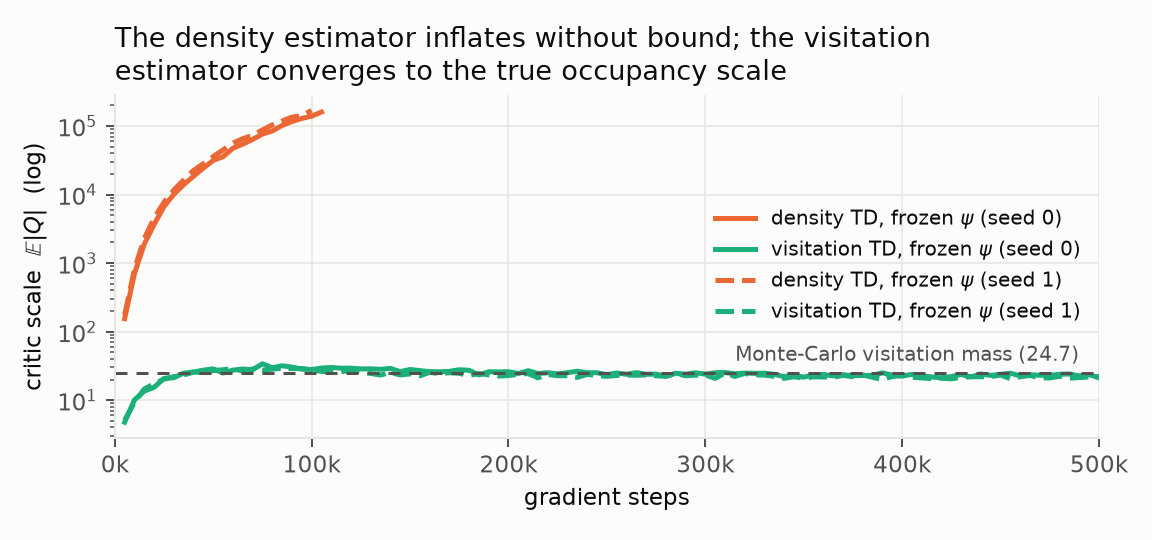
\includegraphics[width=0.66\textwidth]{figures/scale_divergence.png}
\caption{Critic scale $\E|Q|$ (log axis) during visitation-style training on a
\emph{frozen} backward map. The density estimator (orange) inflates without bound
once the orthonormality anchor is removed: its linear term pays unconditionally
for larger values. The bounded region estimator (aqua) plateaus on a Monte-Carlo
estimate of the true discounted visitation mass (dashed), converging to the
target magnitude rather than to a rescaled surrogate.}
\label{fig:diverge}
\end{figure}

The predicted failure occurs (Figure~\ref{fig:diverge}). Within $65$k steps,
critic scale rises from $154$ to $5.4\times10^4$. Control falls from $0.98$ to
$0.60$ and then to $0.42$ by $100$k steps across three seeds. When the backward
map is allowed to update as well, control collapses to $0.07$ and $0.06$ by $50$k
in two runs. Representation corruption accelerates the failure, but the frozen
experiment shows that it is not the original cause.

The complementary ablation keeps orthonormality. Scale remains bounded, but native
success is only $0.225$. A tuned vanilla-FB implementation reaches approximately
$0.42$, still far below the matched goal-conditioned IQL anchor at $0.928$. The
standard estimator therefore faces a practical choice between unstable scale and
restricted control geometry.

\begin{table}[t]
\centering\small
\begin{tabular}{l c c l}
\toprule
Estimator & Matched term & Ortho. & Outcome \\
\midrule
Density surrogate, frozen $B$ & linear & no & scale $154\to5.4\times10^4$ \\
Density surrogate, controlled & linear & yes & success $0.225$ \\
Tuned vanilla FB & linear & yes & success $\approx0.42$ \\
Matched GC-IQL & finite & no & success $0.928$ \\
\bottomrule
\end{tabular}
\caption{The standard density objective needs orthonormality to control scale, but
its stabilized form remains far below the matched goal-conditioned anchor on
\texttt{cube-single}. The frozen experiment isolates the estimator from
representation learning.}
\label{tab:estimator-failure}
\end{table}

\begin{finding}
The failure is not evidence that a rank-$50$ bilinear representation cannot encode
manipulation reachability. It occurs after the backward representation is frozen
at a checkpoint that already supports $0.97$ control. The point-density estimator
itself cannot simultaneously obtain a stable scale and preserve useful control
geometry.
\end{finding}

% ============================================================================
\section{Finite regions turn density matching into Bellman regression}
\label{sec:bounded}

The previous section identifies the missing ingredient: the matched successor
needs a finite target. Querying a region instead of a point supplies one.

\subsection{The bounded substitution}
\label{sec:substitution}

Define the region-hit event
\begin{equation}
\label{eq:hit}
h(s',g)
=
\ind{\|\cube(s')-\cube(g)\|\le\epsilon}
\in\{0,1\}.
\end{equation}
We replace the singular immediate density ratio with this finite event,
\begin{equation}
\label{eq:substitution}
\frac{\delta_{s'}(x)}{\rho(x)}
\quad\longrightarrow\quad
h(s',g).
\end{equation}
Every state--query pair now has an explicit target. The matched pair no longer
needs a separate linear term, and scale is set by a $0/1$ event rather than by a
constraint on the backward representation. The learning problem changes from
point-density estimation to Bellman regression on finite sets.

For a batch, let
\begin{equation}
Q_{ij}=F(s_i,a_i,\psi(g_j))^{\top}\psi(g_j)
\end{equation}
for the diagonal goal-reaching phase. The loss is an ordinary full-matrix
regression,
\begin{equation}
\label{eq:matrix-loss}
\mathcal{L}
=
\frac{1}{n^2}\sum_{i,j}
\left(Q_{ij}-y_{ij}\right)^2,
\end{equation}
optionally normalized by a stop-gradient estimate of the squared prediction
magnitude. There is no diagonal mask and no separate regularizer on $\psi$.

\subsection{Absorption separates reaching from visitation}
\label{sec:backups}

A finite event admits two natural Bellman backups,
\begin{align}
\label{eq:backups}
y^{\Reach}_{ij}
&=
h_{ij}+\gamma(1-h_{ij})\bar Q_{ij},
\\
y^{\Visit}_{ij}
&=
h_{ij}+\gamma\bar M_{ij}.
\end{align}
The reaching backup stops after first arrival. The visitation backup continues to
accumulate every discounted return to the region.

\begin{proposition}
\label{prop:fixed-points}
For a fixed continuation policy, both operators in
Equation~\ref{eq:backups} are $\gamma$-contractions in the sup norm. Their unique
fixed points are
\begin{align}
Q^{\Reach}(s,a,g)
&=
\E\left[\gamma^{T_g}\ind{T_g<\infty}\mid s_0=s,a_0=a\right],
\\
M^{\Visit}(s,a,g)
&=
\E\left[\sum_{t\ge0}\gamma^t h(s_{t+1},g)
\mid s_0=s,a_0=a\right],
\end{align}
where $T_g$ is the first transition whose successor enters $B_\epsilon(g)$.
\end{proposition}

\paragraph{Interpretation.}
$Q^{\Reach}$ is a probability-like goal-reaching value in $[0,1]$. It only needs
to distinguish actions by whether and how quickly they reach a region.
$M^{\Visit}$ is a discounted occupancy quantity in $[0,1/(1-\gamma)]$. It retains
revisit mass and is the object needed for linear reward integration. Success on
the reaching objective therefore does not by itself establish that a successor
measure has been learned.

\subsection{A two-phase training procedure}

We first train the absorbing reaching objective. We then warm-start the visitation
objective from that checkpoint and freeze the backward map $\psi$ so that any new
failure is attributable to the visitation backup rather than to a moving goal
geometry. In the separated phase, the continuation-policy task $z$ and the queried
goal $g$ are sampled independently,
\begin{equation}
M(s,a,z,g)=F(s,a,z)^{\top}\psi(g).
\end{equation}
Reward transfer later supplies $z=z_r$ while integrating over $g$.

The curriculum is empirical rather than mathematically necessary. An earlier
motivation used the renewal identity ``occupancy equals reaching times
recurrence.'' That identity is exact for singleton goals but only approximate for
regions. On this dataset, the estimated recurrence factor has action-wise
intraclass correlation only $0.24$--$0.29$, below a pre-registered threshold of
$0.9$. We therefore use the two phases as an optimization procedure and do not
base the method on the renewal factorization.

\subsection{The bounded target removes the scale--geometry tradeoff}

On \texttt{cube-single}, the bounded objective without orthonormality reaches
$0.967$ success. This more than doubles tuned vanilla FB at approximately $0.42$
and matches or slightly exceeds the matched GC-IQL anchor at $0.928$. Because all
cells use the same actor class, this comparison isolates the value objective more
closely than a comparison between unrelated agents.

\begin{table}[t]
\centering\small
\begin{tabular}{l c c c}
\toprule
Objective & explicit immediate target & orthonormality & success \\
\midrule
Standard FB surrogate & no & standard & $\approx0.42$ \\
Controlled standard surrogate & no & yes & $0.225$ \\
Bounded reaching regression & yes & no & $\mathbf{0.967}$ \\
Matched GC-IQL anchor & yes & no & $0.928$ \\
\bottomrule
\end{tabular}
\caption{A finite region event supplies the scale anchor directly. The bounded
objective no longer needs the geometric constraint that stabilizes standard FB.}
\label{tab:bounded-main}
\end{table}

\begin{finding}
The useful change is not a larger network or a different actor. Replacing the
singular matched-state term with a finite event turns the objective into standard
Bellman regression and removes the need for orthonormality. On
\texttt{cube-single}, this changes the same broad representational family from a
weak controller into a near-saturated one.
\end{finding}

% ============================================================================
\section{Reaching transfers across manipulation; visitation does not come for free}
\label{sec:suite}

The \texttt{cube-single} result leaves two questions. Does bounded reaching work
outside the environment that motivated it? Does the visitation phase preserve the
same control performance?

We evaluate both backups on the four OGBench state-based manipulation environments
for which a tuned vanilla-FB result was available. The GC-IQL anchor is matched in
data, actor class, critic rank, and training budget.

\begin{table}[t]
\centering\small
\begin{tabular}{l c c c}
\toprule
Environment & reaching (phase 1) & visitation (phase 2) & GC-IQL anchor \\
\midrule
\texttt{cube-single} & $\mathbf{0.967}$ & $0.940$ & $0.928$ \\
\texttt{cube-double} & $\mathbf{0.549}$ & $0.358$ & $0.265$ \\
\texttt{scene}       & $\mathbf{0.484}$ & $0.342$ & $0.281$ \\
\texttt{puzzle-3x3}  & $0.200$ & $0.198$ & $0.117$ \\
\bottomrule
\end{tabular}
\caption{Overall success at $500$k steps, using $2$--$3$ seeds. The
\texttt{puzzle-3x3} result is degenerate: every seed succeeds on task 1 and fails
on tasks 2--5, so no method solves the multi-task benchmark.}
\label{tab:suite}
\end{table}

The reaching backup exceeds the matched anchor on all four reported environments.
The most informative differences occur away from the near-ceiling
\texttt{cube-single} task: $0.549$ versus $0.265$ on \texttt{cube-double}, and
$0.484$ versus $0.281$ on \texttt{scene}. These comparisons suggest that bounded
first-arrival supervision is not merely exploiting an idiosyncrasy of the
single-cube benchmark.

The visitation phase tells a different story. It remains above the anchor in every
reported environment, but loses $0.191$ relative to reaching on
\texttt{cube-double} and $0.142$ on \texttt{scene}. On \texttt{cube-single}, the
cost is only $0.027$. Thus the visitation phase is not broken, but neither is it a
free conversion from a strong goal-reaching value into a general occupancy
object.

The distinction matters for the paper's scope. The result that generalizes most
cleanly across environments is the reaching result. The measure-side results in
the following sections are currently established only on \texttt{cube-single},
where the visitation conversion happens to preserve most of the controller's
performance.

\begin{finding}
Bounded reaching is the broad result: it improves over the matched
goal-conditioned anchor throughout the reported suite. Visitation is the more
ambitious object and the less stable one. It still outperforms the anchor, but it
sacrifices a substantial part of the reaching advantage on the harder
environments.
\end{finding}

% ============================================================================
\section{A successful controller does not certify a successor measure}
\label{sec:measure-validity}

A goal-conditioned actor only needs the critic to order actions at the current
state. A successor measure must satisfy stronger requirements across query sets.
We therefore evaluate the phase-2 object directly rather than inferring its
quality from task success.

\subsection{Reaching and visitation induce different action orderings}

Across a grid of $24$ states, $150$ goals, and $16$ actions, the reaching and
visitation critics choose the same greedy action only $29.5\%$ and $29.9\%$ of the
time across two seeds. Chance agreement is $6.25\%$. The agreement is therefore
nontrivial but far below the $0.9$ expected if the two objects induced essentially
the same controller. This confirms that reaching success cannot be used as a proxy
for visitation quality.

\subsection{The deployed object predicts coarse set mass}
\label{sec:set-calibration}

We compare predicted mass on random boxes with Monte-Carlo occupancy of the same
boxes under the policy being scored. The evaluation uses $32$ start states, three
rollouts per start, and horizon $H=200$. The region denominator is computed in two
ways. Exact empirical counts $\rho(B_\epsilon(g))$ isolate the scale of the learned
$M$. A trained density head $\hat N(g)$ evaluates the deployed composition
$M/\hat N$.

\begin{table}[t]
\centering\small
\begin{tabular}{c c c c c}
\toprule
& & \multicolumn{2}{c}{model / MC} & \\
\cmidrule(lr){3-4}
half-width & MC mass & exact $\rho$ & trained $\hat N$ & Spearman \\
\midrule
$0.4$ & $0.56/0.86$ & $3.22/2.03$ & $1.94/1.22$ & $+0.31/+0.33$ \\
$0.8$ & $5.98/5.82$ & $1.92/2.08$ & $\mathbf{1.10/1.16}$ & $+0.68/+0.72$ \\
$1.6$ & $27.4/28.1$ & $2.33/2.18$ & $\mathbf{1.23/1.14}$ & $+0.85/+0.82$ \\
\bottomrule
\end{tabular}
\caption{Set-mass calibration of the phase-2 object, reported per seed. At the
two coarser scales, the deployed composition is within $10$--$23\%$ of truncated
Monte-Carlo occupancy and preserves useful ordering across boxes.}
\label{tab:calib}
\end{table}

At half-widths $0.8$ and $1.6$, the deployed composition has model-to-Monte-Carlo
ratios between $1.10$ and $1.23$ and Spearman correlations between $0.68$ and
$0.85$. The model predicts infinite-horizon discounted mass, whereas Monte Carlo
stops at $H=200$ and omits $\gamma^H=0.134$ of the geometric tail. Multiplying the
reported ratios by $1-\gamma^H=0.87$ brings them close to one.

This result has three limits. First, with exact region frequencies, the same
learned object is $1.9$--$3.2$ times too large. The trained density head
under-corrects one bias with another; it overpredicts region density by $28\%$ in
the direction that improves the final ratio. Second, calibration is weakest at
the smallest evaluated scale, which is also the training-kernel scale. Third,
these measurements are from one environment. The supported statement is that the
deployed composition predicts coarse discounted set mass on
\texttt{cube-single}, not that the raw bilinear object is globally calibrated.

\subsection{Pointwise, the object violates non-negativity}

A successor measure must be non-negative. Over eight draws of $(s_0,a_0,z)$ per
seed and $100$k query goals,
\begin{equation}
\Pr[M(s_0,a_0,z,g)<0]=45.0\%/45.9\%.
\end{equation}
Aggregate box mass can still be accurate because positive and negative entries
cancel inside a set. This explains how coarse calibration and pointwise invalidity
can coexist.

A one-sided penalty
\begin{equation}
\lambda\E\left[\mathrm{relu}(-M)^2\right]
\end{equation}
reduces the negative fraction from $45\%$ to $3.1\%$ at $\lambda=1$ and to $0.7\%$
at $\lambda=10$, without reducing native task success. The repair does not
conserve mass. At half-width $0.8$, aggregate mass grows to $2.5$--$3.6$ times the
Monte-Carlo value, compared with $1.10/1.16$ without the penalty. We therefore do
not adopt it.

\begin{finding}
The visitation representation contains useful coarse occupancy information, but
it is not a valid pointwise successor-measure density. Learned normalization gives
reasonable mass on large boxes, while $45\%$ of individual state--goal values are
negative. Enforcing the sign constraint without a conservation mechanism destroys
mass calibration.
\end{finding}

% ============================================================================
\section{Unseen rewards expose both composition and bandwidth limits}
\label{sec:reward-transfer}

The previous section evaluates occupancy directly. The operational promise of a
successor measure is stronger: it should convert a new reward into a useful value
function and policy without fitting another critic.

\subsection{A transfer harness over the supplied abstraction}

All transfer rewards are functions of cube position, and reward centers are drawn
from dataset states so that every reward lies on observed support. We use six
families with eight instances each:
\begin{itemize}
    \item indicator balls with radii $0.4$, $0.8$, and $1.6$ in normalized
    observation units;
    \item Gaussian rewards with bandwidths $0.4$ and $0.8$;
    \item a two-zone reward containing two disjoint balls separated by more than
    $1.6$.
\end{itemize}
The two-zone family cannot be expressed by a single goal. It therefore provides a
basic test of whether the separated representation can combine rewarded regions.

For each reward, we infer a task vector from $m=10{,}000$ relabeled rows using the
plain moment readout in Equation~\ref{eq:reward-moment}. We use no ridge penalty,
no density correction, and no policy selection over candidate vectors. This
minimal pipeline tests what the representation and its trained policy already
support.

We report
\begin{equation}
\label{eq:gap}
\frac{G_{z_r}-G_{\mathrm{floor}}}
{G_{\mathrm{ceil}}-G_{\mathrm{floor}}}
\end{equation}
against a random-$z$ floor and an oracle proxy that uses the goal embedding of the
dataset state nearest the reward center. We also normalize against the return of
the offline behavior data. The oracle is not the true optimum, especially for
broad or multimodal rewards. Values above one therefore mean that the inferred
policy exceeds this single-goal proxy, not that it exceeds an optimal policy.

\begin{table}[t]
\centering\small
\begin{tabular}{l c c c c}
\toprule
& \multicolumn{2}{c}{prediction} & \multicolumn{2}{c}{control gap} \\
\cmidrule(lr){2-3}\cmidrule(lr){4-5}
Family & Spearman & scale & vs. random $z$ & vs. behavior \\
\midrule
\textsc{ball} $0.4$   & $0.85/0.90$ & $0.014$ & $0.87/0.74$ & $0.80$ \\
\textsc{ball} $0.8$   & $0.80/0.81$ & $0.023$ & $0.70/0.61$ & $0.65$ \\
\textsc{twozone}      & $0.73/0.69$ & $0.017$ & $\mathbf{0.83/0.89}$ & $\mathbf{0.86}$ \\
\textsc{smooth} $0.4$ & $0.75/0.86$ & $0.019$ & $0.54/0.46$ & $0.52$ \\
\textsc{smooth} $0.8$ & $0.62/0.75$ & $0.018$ & $0.23/0.08$ & $0.32$ \\
\textsc{ball} $1.6$   & $0.72/0.81$ & $0.018$ & $-0.10/0.24$ & $0.44$ \\
\bottomrule
\end{tabular}
\caption{Transfer to $48$ evaluation rewards that were not used to fit the
baseline visitation checkpoint. Prediction scale is mean predicted return divided
by mean Monte-Carlo return.}
\label{tab:l2}
\end{table}

The learned object orders candidate returns well across all families: Spearman
correlation remains between $0.62$ and $0.90$, including cases where control is
weak. Concentrated rewards obtain $0.65$--$0.80$ of the behavior-normalized gap.
The two-zone family is the strongest at $0.86$, which is consistent with linear
combination of two rewarded regions. This result does not yet prove that a single
trajectory exploits both zones; that would require trajectory-level occupancy or
a reward for which visiting both is necessary.

Control weakens as reward support broadens. The $1.6$ indicator ball and the broad
Gaussian are the weakest families, even though return ordering remains useful.
Thus the measure representation can predict distinctions that the trained policy
cannot reliably realize.

\subsection{Comparison against the reaching object and FB's own loss}
\label{sec:cross-method}

Equation~\ref{eq:gap} normalizes each checkpoint against \emph{its own} oracle and
floor. It is therefore a within-method statistic and cannot rank methods: the
oracle ceilings themselves differ across objectives by up to a factor of two on
identical rewards, so an objective with a weaker oracle scores higher while
earning less reward. For cross-method comparison we report absolute discounted
return, running the reaching backup and FB's own loss at matched region support
through the identical harness.

\begin{table}[t]
\centering\small
\begin{tabular}{l c c c c}
\toprule
Objective & \textsc{ball} $0.4$ & \textsc{twozone} & \textsc{smooth} $0.8$ & mean (6 families) \\
\midrule
FB loss, matched support & $1.52$ & $4.96$ & $16.43$ & $13.09$ \\
Bounded reaching         & $10.01$ & $8.45$ & $\mathbf{19.71}$ & $16.75$ \\
Bounded visitation       & $\mathbf{15.57}$ & $\mathbf{15.82}$ & $19.43$ & $\mathbf{20.26}$ \\
\bottomrule
\end{tabular}
\caption{Absolute discounted return earned by the inferred task vector, two-seed
means. Unlike Equation~\ref{eq:gap}, this statistic is comparable across
objectives.}
\label{tab:crossmethod}
\end{table}

The visitation object earns $1.33\times$ the reaching object's return on average
and $1.87\times$ on the two-zone family. The mechanism is visible in the oracle
ceilings: driven to the \emph{same} goal with the answer supplied, the visitation
policy accumulates $1.13$--$2.00\times$ more reward than the reaching policy. A
reaching value saturates on arrival, so its policy arrives and stops; a visitation
policy continues to occupy the rewarded region. The advantage is largest on
concentrated and compositional rewards and vanishes on broad ones ($0.99\times$
and $1.05\times$), which is consistent with this explanation, since a reward
earned by wandering gains nothing from dwelling.

Two caveats. The visitation checkpoint is warm-started from the reaching one and
trained for a further $500$k steps, so it has twice the gradient budget; the
ceiling comparison is less exposed to this because it measures what each policy
class accumulates when handed the goal, but an iso-budget control is still owed.
And FB's own loss at matched support is worst of the three: on two families its
oracle drive earns \emph{less} than a random task vector, so Equation~\ref{eq:gap}
is undefined there rather than merely small, and it supplies no usable readout.

\begin{finding}
The visitation object is not merely a more expensive reaching object: it earns
$1.33\times$ the return on unseen rewards, and the gap traces to dwelling rather
than to arrival. This is the clearest evidence that the nonabsorbing backup buys
the semantics it was introduced for. The comparison is not iso-budget, and all
rewards are defined over the supplied cube-position abstraction.
\end{finding}

% ============================================================================
\section{The scale error identifies a second bottleneck: task-vector coverage}
\label{sec:task-vectors}

The reward experiment contains a regular pattern. Predicted returns have useful
rank correlation, but their magnitudes are only $0.014$--$0.030$ of Monte Carlo in
every reward family. A family-independent scale error suggests a missing measure
factor rather than reward-specific value error.

\subsection{Region mass is not a density}
\label{sec:region-normalization}

The learned query is
\begin{equation}
\widetilde M(s,a,g)=M(s,a,B_\epsilon(g)),
\end{equation}
which is the mass of a region, not the density at its center. Integrating this
quantity over centers double counts overlapping balls and inherits the sampling
density of those centers. A local Monte-Carlo approximation to reward integration
therefore requires division by the region's data mass,
\begin{equation}
\label{eq:nhat}
Q_r(s,a)
\approx
\E_{g\sim\rho}
\left[
 r(g)\frac{\widetilde M(s,a,g)}{N(g)}
\right],
\qquad
N(g)=\rho(B_\epsilon(g)).
\end{equation}
If this factor is omitted, predicted scale should be proportional to the mean
region mass
\begin{equation}
\bar N=\E_g[N(g)].
\end{equation}

\begin{figure}[t]
\centering
\includegraphics[width=0.46\textwidth]{figures/scale.pdf}
\caption{Predicted against Monte-Carlo return for all $48$ transfer rewards,
log--log. The uncorrected readout tracks $y=\bar N x$ for the independently
measured $\bar N=0.0137$, the region-mass factor Equation~\ref{eq:nhat} says it
omits, while the $1/\hat N$-weighted readout tracks $y=x$.}
\label{fig:scale}
\end{figure}

The measured value is $\bar N=0.0137$. The uncorrected prediction scale is
$0.014$--$0.030$, with $0.0136$ on the smallest ball family. Applying
$1/\hat N(g)$ during task inference moves the scale to $0.79$--$2.2$
(Figure~\ref{fig:scale}). The correction therefore explains the dominant global
error, although it does not make every reward family precisely calibrated.

\subsection{Correcting value scale does not improve control}

The density correction improves predicted magnitude but does not improve the
policy. The two-zone control gap falls from $0.86$ to $0.46$, and the $0.8$ ball
falls from $0.65$ to $0.48$. This separates value integration from policy
conditioning. A more accurate task vector is not useful if the actor and
forward representation were never trained on vectors of that form.

The baseline task distribution contains $50\%$ random directions and $50\%$
single-goal embeddings $\psi(g)$. A broad reward vector is an aggregate of many
goal embeddings,
\begin{equation}
z_r=\Pi\!\left(\sum_i r_i\psi(g_i)\right),
\end{equation}
where $\Pi$ denotes task-vector normalization. Such vectors can occupy a different
part of task space from either random directions or individual goal embeddings.
The transfer failure therefore suggests a task-conditioning distribution mismatch.
The evidence at this point does not identify the actor alone, because all
$z$-conditioned components may be affected.

\subsection{Training on aggregate task vectors tests the diagnosis}

We add synthetic reward-derived vectors as a third component of the phase-2 task
distribution, while keeping the phase-1 checkpoint, Bellman objective, and all
other hyperparameters fixed. At mixing fraction $\eta$, the new component samples
\begin{equation}
z=\Pi\!\left(\sum_i r_i\psi(x_i)\right)
\end{equation}
for a random non-negative reward over the batch.

We use two generators. \textsc{kernel} samples balls, Gaussians, and two-zone
functions with random centers and log-uniform scales. It matches the broad
functional families used at evaluation. \textsc{rff} samples
\begin{equation}
r(x)=\mathrm{relu}\!\left(\cos(w^{\top}\cube(x)+\varphi)\right),
\qquad
w\sim\mathcal{N}(0,I)/b,
\end{equation}
which has a different functional form. The RFF arm tests whether improvements
require familiarity with the evaluation reward family or merely exposure to
aggregate task vectors.

\begin{figure}[t]
\centering
\includegraphics[width=\textwidth]{figures/bandwidth.pdf}
\caption{Zero-shot control against the reward's spatial support. Control degrades
as support widens within each family. Adding synthetic reward-derived task vectors
repairs the wide indicator reward and the compositional family, but not the wide
Gaussian. The held-out reward form (\textsc{rff}) performs comparably to the
matched one on the repaired families.}
\label{fig:bandwidth}
\end{figure}

\begin{table}[t]
\centering\small
\begin{tabular}{l c c c c}
\toprule
Family & baseline & \textsc{kernel} $\eta{=}0.25$ & \textsc{kernel} $\eta{=}0.5$ & \textsc{rff} $\eta{=}0.25$ \\
\midrule
\textsc{ball} $0.4$   & $0.80$ & $0.87$ & $0.87$ & $0.79$ \\
\textsc{ball} $0.8$   & $0.66$ & $0.71$ & $\mathbf{0.95}$ & $0.73$ \\
\textsc{twozone}      & $0.86$ & $0.92$ & $\mathbf{1.35}$ & $1.11$ \\
\textsc{smooth} $0.4$ & $0.50$ & $0.49$ & $\mathbf{0.78}$ & $0.55$ \\
\textsc{smooth} $0.8$ & $0.15$ & $0.27$ & $0.33$ & $0.12$ \\
\textsc{ball} $1.6$   & $0.07$ & $\mathbf{0.53}$ & $\mathbf{0.49}$ & $\mathbf{0.55}$ \\
\midrule
mean (all 6)          & $0.507$ & $0.630$ & $\mathbf{0.795}$ & $0.640$ \\
native task success  & $0.887$ & $0.948$ & $0.950$ & $0.930$ \\
set mass at hw $0.8$ & $1.10/1.16$ & $1.10/1.19$ & $1.23/1.31$ & $1.26/1.12$ \\
\bottomrule
\end{tabular}
\caption{Control gap against random $z$ after adding synthetic reward-derived
task vectors during phase 2. Entries are two-seed means. Native task success and
set-mass calibration are guard metrics. Oracle ceilings agree within $3$--$23\%$
across these arms, so Equation~\ref{eq:gap} is comparable among them.}
\label{tab:rewardz}
\end{table}

The matched kernel arm at $\eta=0.5$ raises the mean transfer score from $0.507$
to $0.795$. Native task success improves from $0.887$ to $0.950$, and coarse set
calibration remains similar. The clearest repair is the broad indicator ball,
which rises from $0.07$ to $0.49$--$0.55$ across all synthetic-task arms
(Figure~\ref{fig:bandwidth}). The RFF arm reaches $0.55$ on this family despite
sharing no functional form with the indicator-ball evaluation. For this particular
result, aggregate task-vector coverage matters more than matching the test reward
family.

The repair is incomplete. The broad Gaussian reaches at most $0.33$. Unlike a
bounded indicator, a Gaussian assigns nonzero weight throughout the dataset, so
its task vector averages a much larger fraction of the backward representation.
The results therefore identify aggregate task-vector coverage as one bottleneck,
not the only bottleneck.

The two-zone score of $1.35$ exceeds the single-goal oracle proxy by $35\%$. This
shows that the inferred policy can outperform either single-center proxy on the
multimodal reward. It should not be read as exceeding the true optimal policy, and
trajectory-level evidence is still needed to determine whether both zones are
used.

\begin{finding}
Reward inference and task-conditioned control are distinct problems. Region-mass
normalization repairs value scale but not behavior. Training on aggregate
reward-derived task vectors then repairs broad indicator rewards without harming
native task success or coarse calibration. Broad smooth rewards remain unsolved,
and the intervention has only two seeds.
\end{finding}

% ============================================================================
\section{Related work}
\label{sec:related}

\paragraph{Successor representations and successor measures.}
Successor representations separate reward from dynamics by predicting discounted
future occupancy \citep{dayan1993improving}. Successor measures extend this idea
to continuous spaces, where occupancy is represented as a measure or a density
with respect to a reference distribution \citep{blier2021learning}. FB methods
factorize that density into forward and backward representations and use reward
moments to infer task vectors \citep{touati2021learning,touati2023does}. Our work
keeps the same goal of reward reuse but studies a more basic estimator question:
what happens when the immediate point-density term is not representable as a
finite regression target? Bounded region regression changes the query object from
a point density to finite set mass.

\paragraph{Goal-conditioned offline reinforcement learning.}
Goal-conditioned methods learn values or policies for reaching a supplied goal.
Our matched anchor uses the IQL principle of fitting values conservatively from
offline data \citep{kostrikov2021offline}. The main conceptual difference is that
a diagonal goal-conditioned value only needs to evaluate each goal under its own
policy. A successor measure retains an independent query argument and is expected
to support linear reward composition. Our experiments use this distinction as an
evaluation principle: goal success evaluates reachability, while set calibration
and reward transfer evaluate the measure claim.

\paragraph{Manipulation benchmarks and play data.}
OGBench provides offline navigation and manipulation datasets together with
standardized goal-conditioned evaluations \citep{park2024ogbench}. We focus on
state-based manipulation because it exposes a large gap between FB and a matched
goal-conditioned anchor. The region abstraction used here is supplied from the
benchmark state and success criterion. The method should therefore be understood
as learning over a given outcome structure, rather than discovering task-relevant
object variables from raw observations.

\paragraph{Hitting values versus occupancy.}
The absorbing and nonabsorbing backups correspond to different questions. A
hitting value asks whether and how quickly a region will first be reached.
Occupancy asks how often the process will return afterward. Many manipulation
tasks are evaluated by first reaching a tolerance region, so the reaching object
can be sufficient for control even when the visitation object is inaccurate. Our
experiments make this distinction explicit and show that the two objectives have
different empirical difficulty, and that the difference is visible in reward
transfer as well as in control (Section~\ref{sec:cross-method}).

% ============================================================================
\section{Limitations}
\label{sec:limitations}

\paragraph{The region structure is supplied from the evaluation.}
The abstraction $\cube$ selects three of twenty-eight observation dimensions, and
$\epsilon$ matches the benchmark's success threshold. A control that retains FB's
original loss and changes only the support from a point to the same ball reaches
$0.367$, far below the approximately $0.93$ obtained by bounded regression. Thus
the region alone is not sufficient. The converse experiment has not been run: we
do not know whether the bounded objective remains effective for a point query, a
learned abstraction, or a region unrelated to the evaluation variable. This is
the main unresolved generalization question.

The forty-eight transfer rewards are new reward functions over the same supplied
cube-position abstraction. They do not test transfer to a new state abstraction.
The synthetic-task intervention also uses reward functions over this abstraction.
Its use of ``zero-shot'' refers to held-out evaluation rewards, not to training
without any synthetic reward structure.

\paragraph{The visitation object is not a valid pointwise measure.}
Approximately $45\%$ of evaluated state--goal values are negative. The hinge
penalty reduces sign violations but inflates aggregate mass by $2.5$--$3.6$ times.
We do not have a parameterization that jointly preserves non-negativity, aggregate
mass, and linear dependence on the backward features required by the standard
reward readout.

\paragraph{Measure-side evidence is restricted to one environment.}
Calibration, reward transfer, and task-vector experiments are all performed on
\texttt{cube-single}. The visitation backup loses $0.19$ and $0.14$ relative to
reaching on \texttt{cube-double} and \texttt{scene}. Whether its measure-side
capabilities survive in environments where visitation has a control cost remains
untested.

\paragraph{The transfer harness covers few competing methods.}
Section~\ref{sec:cross-method} compares the visitation object against the reaching
backup and against FB's own loss at matched support in the identical harness. The
goal-conditioned anchor is implemented in a different framework and has not been
run through it, and no external successor-measure baseline has been evaluated on
these forty-eight rewards. The random-$z$ floor is a single draw shared across
rewards, and the oracle proxy understates the achievable return for broad and
multimodal rewards. The results establish internal capabilities and failure modes,
not comparative state of the art in zero-shot reward transfer.

\paragraph{The cross-method comparison is not iso-budget.}
The visitation checkpoint is warm-started from the reaching checkpoint and trained
for a further $500$k steps. Part of the $1.33\times$ return advantage in
Table~\ref{tab:crossmethod} may reflect the additional budget rather than the
backup. The oracle-ceiling comparison is less exposed to this confound, but a
reaching run at matched total budget has not been completed.

\paragraph{The calibrated composition depends on a learned density head.}
The trained $\hat N$ head is biased by $+28\%$ in a direction that improves the
model-to-Monte-Carlo ratio. With exact counts, raw set mass is $1.9$--$3.2$ times
too large. The deployed composition is approximately calibrated on coarse boxes;
the learned $M$ itself is not.

\paragraph{Statistical power is limited.}
Most cells contain two or three seeds. The native task-success increase from
$0.887$ to $0.950$ in the task-vector experiment is suggestive rather than
decisive, as are differences among individual synthetic-reward generators. The
broad indicator improvement is larger and appears in every arm and both seeds,
but it still needs replication.

\paragraph{Claims concern the value objective more than the actor.}
All primary cells use one flow-BC actor class. An actor-isolation sweep with a
different actor reversed the advantage over the anchor at one setting in one
seed. The task-vector intervention changes the training distribution seen by all
$z$-conditioned components, so it establishes a task-conditioning mismatch but
does not isolate the actor as the only cause.

\paragraph{The fixed-policy theory does not cover the full algorithm.}
The contraction result applies to idealized fixed-policy Bellman operators. The
practical method uses a changing actor, a rank-$50$ factorization, twin-min
targets, offline bootstrap actions, and a backward map that was first trained for
reaching. Stability of this estimator is an empirical result rather than a
guarantee for the complete learning system.

% ============================================================================
\section{Conclusion}
\label{sec:conclusion}

The goal of this work was not to begin with a new successor-measure architecture.
It was to understand why a standard successor-measure objective fails on
manipulation data when a matched goal-conditioned value function succeeds. The
answer begins with the estimator. A pointwise successor density has a singular
immediate term, and the standard FB surrogate replaces it with a linear incentive
whose scale must be controlled indirectly through representation geometry. A
frozen-embedding experiment shows that this problem persists even when the
representation already supports strong control.

Finite regions provide the missing target. They turn the immediate term into a
binary event and allow the full state--query matrix to be trained with ordinary
Bellman regression. The absorbing version produces the paper's broadest result:
strong goal-reaching policies across the reported OGBench manipulation suite. The
nonabsorbing version is more demanding. On \texttt{cube-single}, it predicts
coarse occupancy and earns $1.33\times$ the reaching object's return on unseen
rewards, but it is not pointwise non-negative, depends on density normalization,
and loses control performance on harder environments.

The experiments also separate value correctness from policy coverage. Correcting
the region-mass factor repairs predicted return scale without improving behavior.
Training on reward-derived aggregate task vectors then repairs broad bounded
rewards, while broad smooth rewards remain difficult. What emerges is a sequence
of distinct problems: represent a finite outcome, learn its visitation measure,
integrate a new reward, and train a policy that can act on the resulting task
vector. Bounded region regression resolves the first problem and makes measurable
progress on the next three. Discovering the outcome structure and learning a
valid non-negative measure remain open.

\bibliography{references}
\bibliographystyle{iclr2027_conference}

% ============================================================================
\appendix
\section{Additional experimental detail}
\label{app:detail}

\subsection{Divergence: the full control set}
\label{app:diverge}

Section~\ref{sec:frozen-test} reports the frozen-embedding experiment in condensed
form. The complete set of controls:

\begin{itemize}
\item \textbf{Frozen $B$, density estimator.} Critic scale
$154\to5.4\times10^{4}$ within $65$k steps; success decays $0.98\to0.60\to0.42$ by
$100$k (three seeds). The embedding comes from a checkpoint supporting $0.97$
control and is held fixed, so representation quality cannot account for the
outcome.
\item \textbf{Trainable $B$, density estimator.} Collapses faster:
$0.97\to0.07$ and $0.98\to0.06$ by $50$k (two seeds).
\item \textbf{Frozen $B$, bounded region estimator.} Scale plateaus on the
Monte-Carlo estimate of the true discounted visitation mass; both seeds complete
$500$k steps without instability.
\item \textbf{Orthonormality retained.} Scale is bounded, but native success is
$0.225$ --- the other half of the tradeoff of Section~\ref{sec:singular}.
\end{itemize}

\subsection{A tabular instance of the same structure}
\label{app:playpen}

The structural claims of Section~\ref{sec:bounded} can be exhibited exactly in a
$50$-state MDP built with the same anatomy as manipulation play data: a
$7\times7$ grid plus a pit, in which the column is the semantic coordinate (the
region variable) and the row is an interaction mode invisible to the region. A
$2\times2$ sticky bowl models a cube at rest; the top row is a conveyor that
drifts two columns per step regardless of action, modelling a carried cube whose
position cannot be held; riding off its end drops into a hard-to-leave pit.

Fitting a rank-$8$ bilinear $F^{\top}B$ on $20$k offline transitions with
identical architecture and data, the region regression reaches relative error
$0.05$--$0.09$ and per-state goal-ranking correlation $0.96$--$0.99$, while the
density-TD form reaches only $0.38$ and $0.65$; adding the orthonormality
regularizer makes the latter worse ($0.53$ and $0.45$). Two honest notes. With no
actor in the loop, the density estimator fits poorly but does not diverge, which
is consistent with the divergence of Section~\ref{sec:frozen-test} being a
property of the estimator-plus-actor system rather than of the loss alone. And
absorbing-first and direct visitation regression perform alike here ($0.09$ versus
$0.05$), consistent with the curriculum's value lying in the control loop rather
than in policy evaluation.

This environment also exhibits the ranking disagreement that motivates the
visitation backup. Weighting a stable region and a transient one so that they are
nearly equally reachable, ranking by reaching value selects the transient region
while ranking by occupancy selects the stable one; exact policy evaluation
confirms the latter ($96.8$ versus $47.9$ discounted return).

\subsection{Goal-decoding extraction routes}
\label{app:decode}

Earlier versions of this work evaluated a different reward suite through
goal-\emph{decoding} routes: inferring $z_r$, decoding it to a single dataset
state by top-$k$ reward-weighted retrieval, and conditioning the actor on that
state. Those routes reach $0.73$--$0.99$ on every family whose optimum reduces to
one dataset state, and fail on families that do not. Because the outcome is
determined by the decode rather than by the measure, we do not use them in the
main text; the forty-eight-reward suite of Section~\ref{sec:reward-transfer}
consumes $z_r$ directly.

\subsection{Reward construction}
\label{app:rewards}

All transfer rewards are functions of the cube position $\cube(x)$, with centers
drawn uniformly from dataset states. Per family, eight instances:
\textsc{ball}~$\epsilon$ is $\ind{\|\cube(x)-c_0\|\le\epsilon}$ for
$\epsilon\in\{0.4,0.8,1.6\}$ in observation units where the trained kernel is
$0.4$; \textsc{smooth}~$\sigma$ is $\exp(-\|\cube(x)-c_0\|^2/2\sigma^2)$ for
$\sigma\in\{0.4,0.8\}$; \textsc{twozone} is
$\max_k\ind{\|\cube(x)-c_k\|\le0.4}$ with $\|c_1-c_2\|>1.6$. Inference uses
$m=10{,}000$ relabeled rows. Prediction is scored from $12$ teleported starts
$\times$ $2$ rollouts; control is scored over $10$ episodes per drive at horizon
$200$.

The synthetic rewards used to populate the task-vector distribution in
Section~\ref{sec:task-vectors} are drawn per batch element. \textsc{kernel} mixes
balls, Gaussians and two-zone rewards with centers drawn from the batch and
log-uniform radii in $[0.2,2.0]$. \textsc{rff} draws
$r=\mathrm{relu}(\cos(w^{\top}\cube+\varphi))$ with $w\sim\mathcal{N}(0,I)/b$ and
$\varphi\sim\mathrm{U}[0,2\pi)$. Both are normalized before the moment readout;
the projection to the task-vector sphere makes their scale immaterial.

\subsection{Monte-Carlo evaluation protocol}
\label{app:mc}

Teleport-style Monte-Carlo evaluation of the kind used in
Section~\ref{sec:set-calibration} must reset the environment before every rollout,
not merely overwrite the simulator state. The episode step counter otherwise
persists across rollouts and every rollout after the first truncates immediately,
which inflates model-to-Monte-Carlo ratios by one to two orders of magnitude. A
useful invariant when debugging such a harness is that the implied total
Monte-Carlo mass must approach $\sum_k\gamma^k$, since the tracked object is
always somewhere.

\end{document}
